\documentclass[12pt,letterpaper]{article}
\usepackage[a4paper, total={7in, 10in}]{geometry}
\renewcommand{\familydefault}{\sfdefault}
\usepackage{graphicx}
\usepackage{helvet}
\usepackage{authblk}
% \usepackage{hyperref} % you cannot use this when doing the x-ref, but xr--hyper should work
\usepackage{amsmath} 
\usepackage{amssymb} 
\usepackage{orcidlink} 
\usepackage[super,comma,sort&compress]  
   {natbib}\bibliographystyle{numbered}
\usepackage[right]{lineno} \linenumbers
\usepackage{lineno}
\usepackage{xr-hyper} 
\newcommand{\R}[1]{\label{}\linelabel{#1}} % get line #s


\makeatletter
\renewcommand{\maketitle}{\bgroup\setlength{\parindent}{0pt}
\begin{flushleft}
  \textbf{\@title}
  
  \@author
\end{flushleft}\egroup}
\makeatother

%%% JA added
\usepackage{subcaption}



%%%  Insert title below; leave date empty.

\title{Scattered spring: How climate change disrupts the synchrony of biological events}
\date{}

%%%  Author first and last names should be spelled 
%%%  out in their entirety (do not abbreviate "J.H. 
%%%  Watson" unless this is how the author's name 
%%%  always appears). Middle initials are OK. Do 
%%%  not include titles, positions, or degrees.

%%%  Use numbered footnotes to indicate institutional 
%%%  affiliations. Authors may have multiple 
%%%  institutional affiliations, and affiliations 
%%%  may be shared among multiple authors.

%%%  After the institutional affiliations, numbered 
%%%  footnotes may be used to indicate an author's 
%%%  present address, equal contribution status, 
%%%  and/or senior author status. 

%%%  The final numbered footnote should indicate 
%%%  which author is the lead contact (required). 
%%%  One author must be designated as the lead contact. 
%%%  There can be no more than one lead contact. 

%%%  Corresponding authors should be indicated with 
%%%  asterisks (*). Use 2 asterisks (**) for the 
%%%  second-listed corresponding author, 3 (***) for 
%%%  the third-listed, and so on. The lead contact 
%%%  must be a corresponding author. Additional 
%%%  authors may also serve as corresponding authors.

\author[1,5,*,\orcidlink{0000-0003-3772-8030}]{Jonathan Auerbach}
\author[2,3,**,\orcidlink{0000-0002-6975-2601}]{Andrew Gelman}
\author[4,***,\orcidlink{0000-0001-7653-893X}]{E. M. Wolkovich}

%%%  Institutional affiliations should contain the 
%%%  following information at minimum: department(s)/
%%%  subunit(s), institution, city, state/region (if 
%%%  applicable), and country. 

\affil[1]{Department of Statistics, George Mason University, Fairfax, VA USA}
\affil[2]{Department of Statistics, Columbia University, New York, NY USA}
\affil[3]{Department of Political Science, Columbia University, New York, NY USA}
\affil[4]{Forest and Conservation Sciences, University of British Columbia, Vancouver, BC Canada}
\affil[5]{Lead contact}

%%%  List only one email address per corresponding author.

\affil[*]{Correspondence: jauerba@gmu.edu}
\affil[**]{Correspondence: ag389@columbia.edu}
\affil[***]{Correspondence: wolkovic@mail.ubc.ca}

\begin{document}

\maketitle

\section*{SUMMARY}

%%% 150 out of 150 word maximum

Many biological processes, including plant leafout and flowering, occur once cumulative temperatures reach a threshold. An important implication is that higher temperatures cause thresholds to be reached sooner so that the timing of spring events advances earlier in the calendar year as climates warm. But growing evidence has found many cases in which the rate of advancement has slowed and the variance in the timing of spring events has increased as climates have warmed, raising questions about the resilience of temperature-based coordination to anthropogenic climate change. We explain how the threshold process produces these trends using experimental and real-world data. As temperatures continue to increase, we find springtime events will become less synchronized and more variable. By 2100, our results predict much of the American South will experience a scattered spring under a high-warming scenario, \R{why}with the potential for disrupted crop and wild species pollination, and other major mismatches in springtime events. % with the average time between spring flowering events increasing by several weeks in many locations. 

\section*{KEYWORDS}

%%%  Include up to 10 keywords, separated by commas. 
%%%  Keywords entered in EM are not carried over; only 
%%%  keywords included in the main text will be used 
%%%  in the final article metadata. Please note that 
%%%  for some journals, keywords are chosen by the editors.

phenology, climate change, statistical methodology, stopping times, variance estimation

\section*{INTRODUCTION}

Many biological events are triggered not by temperature on a single day, but by temperature accumulated over many days \citep{larcher1980}. The long-standing and widespread `thermal-sum' model states that the bud of a flowering plant, for example, first blooms in the spring once cumulative temperatures exceed a plant-specific threshold \citep{quetelet1849letters, chuinearees}.\R{alreadycited1} This mechanism is thought to synchronize a wide variety of seasonal events within an ecosystem---for instance, ensuring that pollinators emerge when flowers are in bloom  \citep{schwartzbook}.\R{scatteredspring1} It also supports an array of forecasting tools in which scientists track cumulative temperatures or `growing degree days' to predict harvest dates, manage pest emergence, and assess how changing temperature patterns reshape ecological communities \citep{schwartzbook}.

Shifts in the timing of biological events have been among the clearest fingerprints of anthropogenic climate change across both natural and managed systems \citep{ipcc2022}. But researchers have struggled to fully predict or explain these shifts in recent years. One puzzle is that while the timing of many biological events has moved earlier (i.e., advanced) as climates warm, the rate of advancement has slowed \citep{fu2015declining}. We refer to this pattern in which events appear less sensitive to additional warming as `declining sensitivity.'

A second puzzle is that the variance in the timing of biological events has in some cases declined and in others increased \citep{vitasse2018global,stemkovski2023disorder}. Higher variance has also manifested as previously unknown or rare events becoming more common \citep{chuine2025living}. We refer to this pattern in which events appear less coordinated as `declining synchrony.'

Declining sensitivity and synchrony are almost always interpreted as evidence that the long-standing and widespread thermal-sum model is wrong or incomplete. Researchers have suggested myriad complexities or alternatives \citep{fu2015declining,wolkovich2021simple,gao2024thermal}. % emwOct: This could be a place to sneak in Clark, Keenan, and us if you think you need to ... 
Yet no work has examined whether these puzzles are explained by the thermal-sum model, or how sensitivity and synchrony will continue to evolve under the thermal-sum model as climates continue to warm.

Here we show that the thermal-sum model is an example of a stopped random walk, and we build a simple and transparent framework for the analysis of biological event times using statistical tools developed for stopped random walks. Applying the framework to observational and experimental plant\R{scatteredspring2} data, we find that the thermal-sum model explains both declining sensitivity and synchrony. Thus modifications and alternative approaches often suggested  \citep{fu2015declining,vitasse2018global} may be unnecessary and yield inaccurate predictions. In contrast to predictions from current models of biological events for many plants and animals,\R{scatteredspring3}\cite{chuinearees} our framework implies that as springtime events advance with anthropogenic warming, they enter a new temperature regime in which the typical time between events in the same ecosystem can increase from a few days to a month or more, a phenomenon we refer to as a `scattered spring.'


\section*{RESULTS AND DISCUSSION}

The thermal-sum model states that a biological event occurs when cumulative temperature reaches a threshold. This model is an example of a stopped random walk where the cumulative temperature is the position of the walk, and the biological event occurs when the walk arrives at the threshold. 

Consider the timing of a specific biological event, such as the bloom date of a bud. Let $X_i$ denote the effective temperature experienced by that bud on day $i$. We model $X_i$ under two temperature regimes (Figure \ref{fig:model}).

\begin{figure*}[t]
\centering
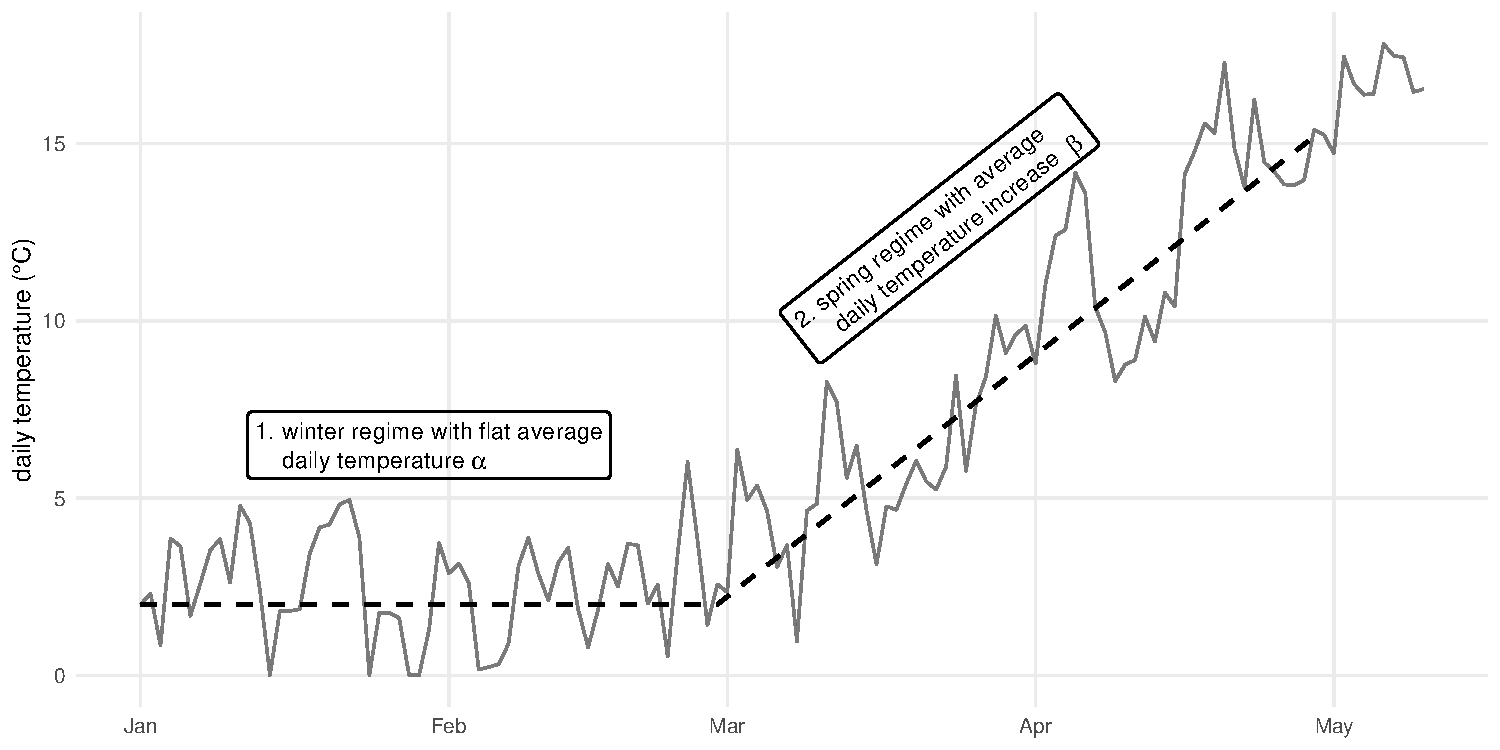
\includegraphics[width=0.9\textwidth]{figure-latex/two_regimes.pdf}
\caption{We model the daily temperature (solid line) as trend (dashed line) plus noise. The timing of springtime events in temperate climates depends on whether temperature is accumulated during one of two regimes, 1. the winter regime (relatively flat average daily temperature near the winter solstice, which we refer to as the `winter temperature' or $\alpha$), or 2. the spring regime (relatively linear average daily temperatures near the spring equinox, the slope of which we refer to as `spring warming' or $\beta$). We assume the effective temperature experienced by the bud is positive since biological limits prevent plants from accumulating very low forcing temperatures, taken here to be $0^{\circ}$C \citep{larcher1980} although this is easily adjusted.}
\label{fig:model}
\end{figure*}

The first regime is the `winter regime' in which the average daily temperature is approximately constant at some level $\alpha>0$. This regime is often observed in the winter months following the solstice, and we refer to $\alpha$ as the `winter temperature.'  The second regime is the `spring regime' in which the average daily temperature rises at a constant rate $\beta>0$. This regime is often observed in the spring months closer to the equinox, and we refer to $\beta$ as `spring warming.' 

In either regime, the effective temperature is modeled as the average temperature plus noise $\epsilon_i$. That is, $X_i = \alpha + \beta i + \epsilon_i,$ where $\beta=0$ in the winter regime and $\beta>0$ in the spring regime. We assume the $\epsilon_i$ are independent with mean $0$ and variance $\sigma^2$.

Noise in this formulation can represent the influence of various biological factors, depending on the scale of analysis and on our evolving understanding of what triggers springtime events. At the bud level, it represents idiosyncratic variation specific to that bud, which could arise from microclimate differences \citep{schwartz2014separating}, bud color variation \citep{peaucelle2022accurate}, or internal biological differences that affect when the bud begins accumulating temperatures \citep{vanderschoot2014,pan2023epigenetic}.

This two regime model in which average temperatures switch from constant to increasing well-describes both historic springtime temperature data (Figure S1 in SI.3) and projected springtime temperature data (Figure S4 in SI.3). Here we assume that warming occurs entirely in one of the two regimes, although similar results hold when warming occurs under both regimes (since in such cases the spring regime dominates, see SI.1 for details.)

The bloom date $\nu(\tau)$ is the day $n$ on which the cumulative temperature $\sum_{i=1}^n X_i$ first reaches a plant-specific threshold $\tau>0$. This formulation is standard in growing degree day models and, more generally, the `forcing' component of many process-based models of plant phenology \citep{schwartzbook}. This formulation also allows us to use standard results for stopped random walks, which yield asymptotically normal approximations for the bloom date when the threshold is sufficiently large that accumulation occurs over many days.

In the winter regime, average temperatures are constant during accumulation ($\beta = 0$), and cumulative average temperatures grow at an approximately linear rate. The average bloom date advances with climate change in step with the winter temperature ($\mathbb{E}[\nu(\tau)] \approx \tau / \alpha$) as is often described in the literature \citep{vitasse2022great}. In the spring regime, average temperatures increase during accumulation ($\beta > 0$), and cumulative average temperatures grow quadratically. In this regime, the average bloom date squared advances in step with spring warming ($\mathbb{E}[\nu(\tau)] \approx \sqrt{ 2 \tau / \beta}$). 

Within either regime, the relationship between the average bloom date and temperature is non-linear as observed\R{nomorerecent} \citep{fu2015declining,wolkovich2021simple}. Indeed, both regimes predict declining sensitivity in that the average bloom date advances at a diminishing rate when warming increases as measured by the winter temperature ($\alpha$) or spring warming ($\beta$).

Importantly, the effects of warming within the two regimes make very different predictions regarding the synchrony of events---that is, the variance in the timing of events within the same year and location due to idiosyncratic differences described above such as microclimate. Both predict decreased variance with warming ($\mathrm{Var}(\nu(\tau)) \approx \sigma^2 \, \tau / \alpha^3$ in the winter regime and $\mathrm{Var}(\nu(\tau)) \approx \sigma^2 / \sqrt{2 \beta^{3} \tau}$ in the spring regime). But the overall size of the variance depends on whether the threshold $(\tau)$ is in the numerator or the denominator.

When the threshold is in the denominator as in the spring regime, the variance is small, reflecting the fact that as temperatures accumulate, noise is quickly overwhelmed by the signal (quadratic increase in cumulative average temperatures). This is how temperatures near the equinox synchronize plants (and buds within plants, alongside many other plant and animal organisms)\R{scatteredspring4} with the same threshold---by making idiosyncratic differences such as microclimate negligible. In contrast, when the threshold is in the numerator as in the winter regime, the variance is large, reflecting the fact that noise remains relatively influential (compared to the linear increase in cumulative average temperatures) and idiosyncratic differences translate into larger differences in threshold-crossing times. 

In this way, our results reveal the key mechanism that determines whether synchrony declines: the temperature regime under which accumulation occurs. When average temperatures increase day over day, as they often do near the equinox, springtime events tend to be tightly synchronized. But when warming shifts those events closer to the solstice, where average temperatures are comparatively constant, event times become more variable. The shift in regimes is observable as a `scattered spring' in which, as springtime events advance, they become less synchronized. 

Our results show that the two most important aspects of temperature are the levels of winter temperature $(\alpha)$ and spring warming $(\beta)$. This simplification yields a simple and transparent framework for translating spatially varying climate change into spatially varying predictions of both the advancement of spring and its variability. 

To demonstrate the framework, we analyze bloom dates from the lilac--honeysuckle phenology network, compiled by \cite{rosemartin2015lilac} from sites across the continental United States between 1956--2014. We limit our analysis to the purple common lilac (\textit{Syringa vulgaris}) and the phenophase full bloom, and we update the dataset using USA National Phenology Network records from the same sites and species until 2025 \citep{switzer_etall:2025}. For each record, we estimate the winter temperature $(\alpha)$ and spring warming $(\beta)$. We then estimate the conditional mean and standard deviation functions of the bloom date using a generalized additive model \citep{hastie1986generalized, wood2017generalized}. 

We find that increasing either the winter temperature, spring warming, or both has shifted lilac flowering times exactly as predicted by the thermal-sum model (Figures \ref{fig:lilac_te}). Warming in either regime (increasing $\alpha$ or $\beta$) leads to earlier mean bloom dates, which advance at a decreasing rate (declining sensitivity). Warming in the winter regime only (increasing $\alpha$ and holding $\beta$ fixed) returns greater variance (higher standard deviation, declining synchrony), while warming in the spring regime only (increasing $\beta$ while holding $\alpha$ fixed) returns lower variance (lower standard deviation, increasing synchrony). This is the `scattered spring' predicted by the model: in the first case, plants are more likely to accumulate their thermal sum in the winter regime, which results in the larger variance.

\begin{figure*}
    \centering

    \begin{subfigure}[b]{0.9\textwidth}
        \centering
        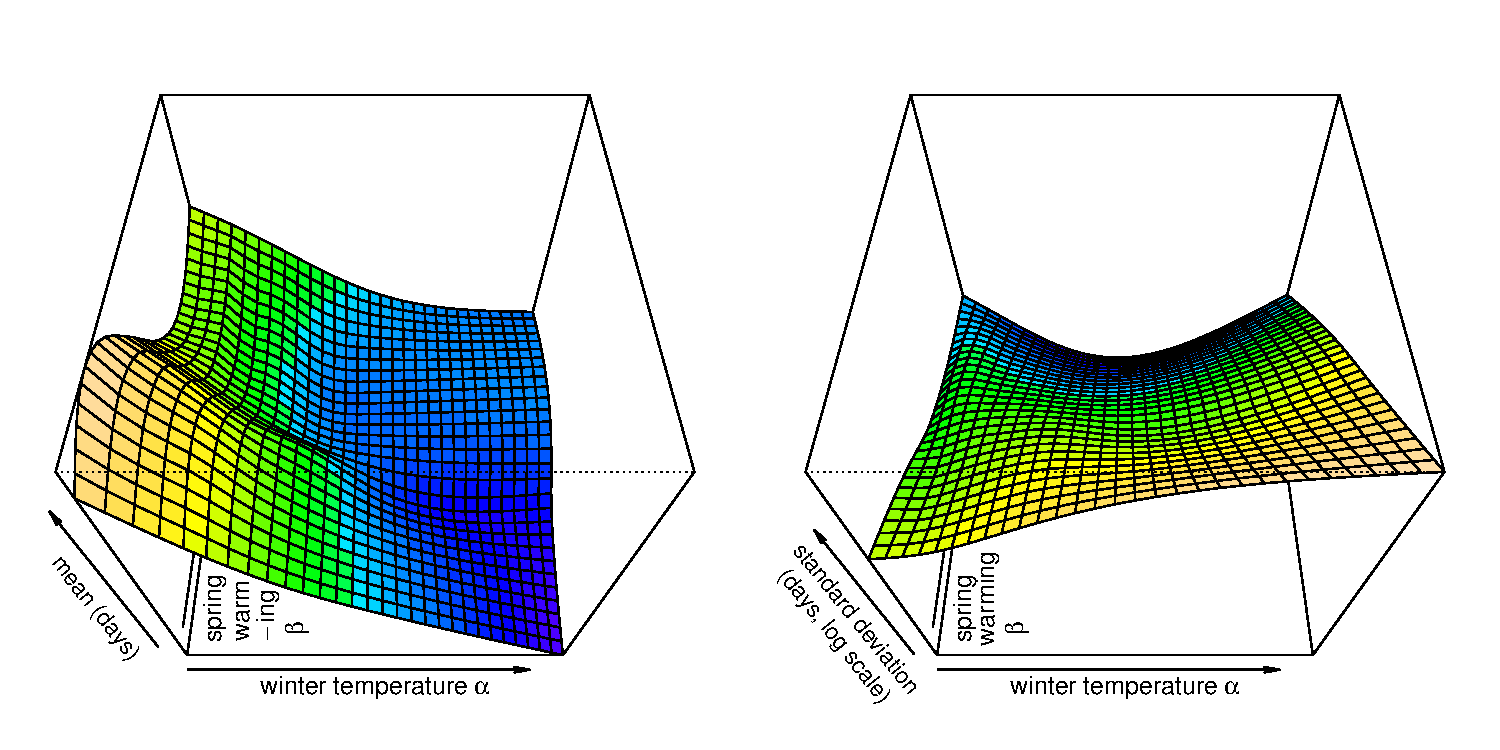
\includegraphics[width=1\linewidth]{figure-latex/lilac_te_mean-1}
        \caption{Bivariate plots showing mean (left) and log standard deviation (right) of lilac bloom dates as a function of winter temperature (\(\alpha\)) and spring warming (\(\beta \)).}
    \end{subfigure}

    \vspace{0.5em}

    \begin{subfigure}[b]{0.9\textwidth}
        \centering
                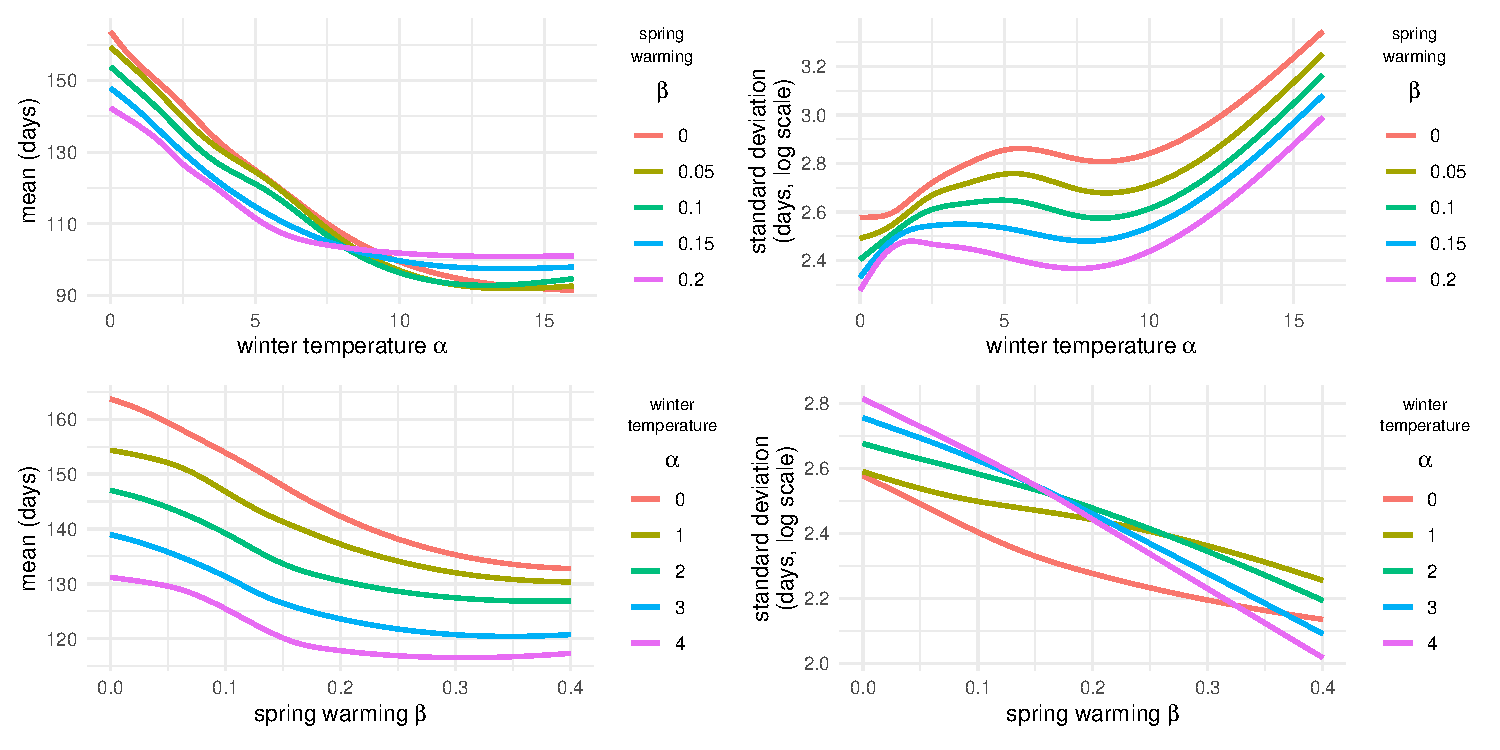
\includegraphics[width=1\textwidth, trim=0 0 .85in 0, clip]{figure-latex/lilac_te_mean-2_t}
        \caption{Cross-section plots showing mean (left) and log standard deviation (right) of lilac bloom dates as a function of winter temperature (\(\alpha\)) holding spring warming (\(\beta \)) constant (top) and as a function of spring warming (\(\beta \)) holding winter temperature (\(\alpha\)) constant (bottom).}
    \end{subfigure}

     \caption{Mean and log standard deviation of lilac bloom dates (n = 10,613 from Rosemartin et al. 2015, updated to 2025 using USA National Phenology Network records) by winter temperature $(\alpha)$ and spring warming $(\beta)$ as estimated by a generalized additive model. The estimated functions are shown using bivariate plots (a, top) and cross-section plots (b, bottom). The bivariate plots show the mean decreases as $\alpha$ and $\beta$ increase (left), while the standard deviation can increase or decrease depending on the relative values of $\alpha$ and $\beta$ (right). The cross-section plots show the mean decreases both as \(\alpha\) increases holding \(\beta\) constant (top left) and as \(\beta\) increases holding \(\alpha\) constant (bottom left), while the standard deviation increase when \(\alpha\) increases holding \(\beta\) constant (top right) and decreases when \(\beta\) increases holding \(\alpha\) constant (bottom right). Temperature is measured in $^\circ$C.}
    \label{fig:lilac_te}
\end{figure*}
 

In this way, the thermal-sum model explains a wide variety of trends in the mean and variance of biological event times, challenging a growing body of work claiming such trends either invalidate the model or justify additional complexity \citep[e.g.,][]{fu2015declining,kovaleskipreprint}. For example, researchers have suggested that warming may influence effects of photoperiod or chilling (cool temperatures required to break endodormancy), which in turn change the threshold of the thermal sum.\citep[e.g.,][]{piao2017,meng2020}.\R{addedcites1} %emwOct: I switched to warming instead of climate change here since one citation is on urban heat islands

We show that these additional factors are unnecessary by applying our framework to rare experimental data in which photoperiod and chilling are held fixed but forcing temperatures vary. We use results from \cite{Charrier:2011aa}, who tested the effect of different constant temperatures on walnut (\textit{Juglans regia} and \textit{Juglans regia x nigra} hybrids) tree budburst after the plants had experienced sufficient chilling to break endodormancy (385 buds were observed on stems sampled from 15 trees, chilled at \(4^\circ\)C), and we fit the winter regime approximation to the thermal-sum model (since temperatures are held constant, this experiment replicates this regime) using weighted least squares. The data exhibit the exact nonlinear relationship in the mean and variance as predicted by the thermal-sum model (Figure \ref{fig:experiment}), establishing the sufficiency of the model even under an extreme temperature range and controlled chilling and photoperiod conditions. 

\begin{figure*}[t]
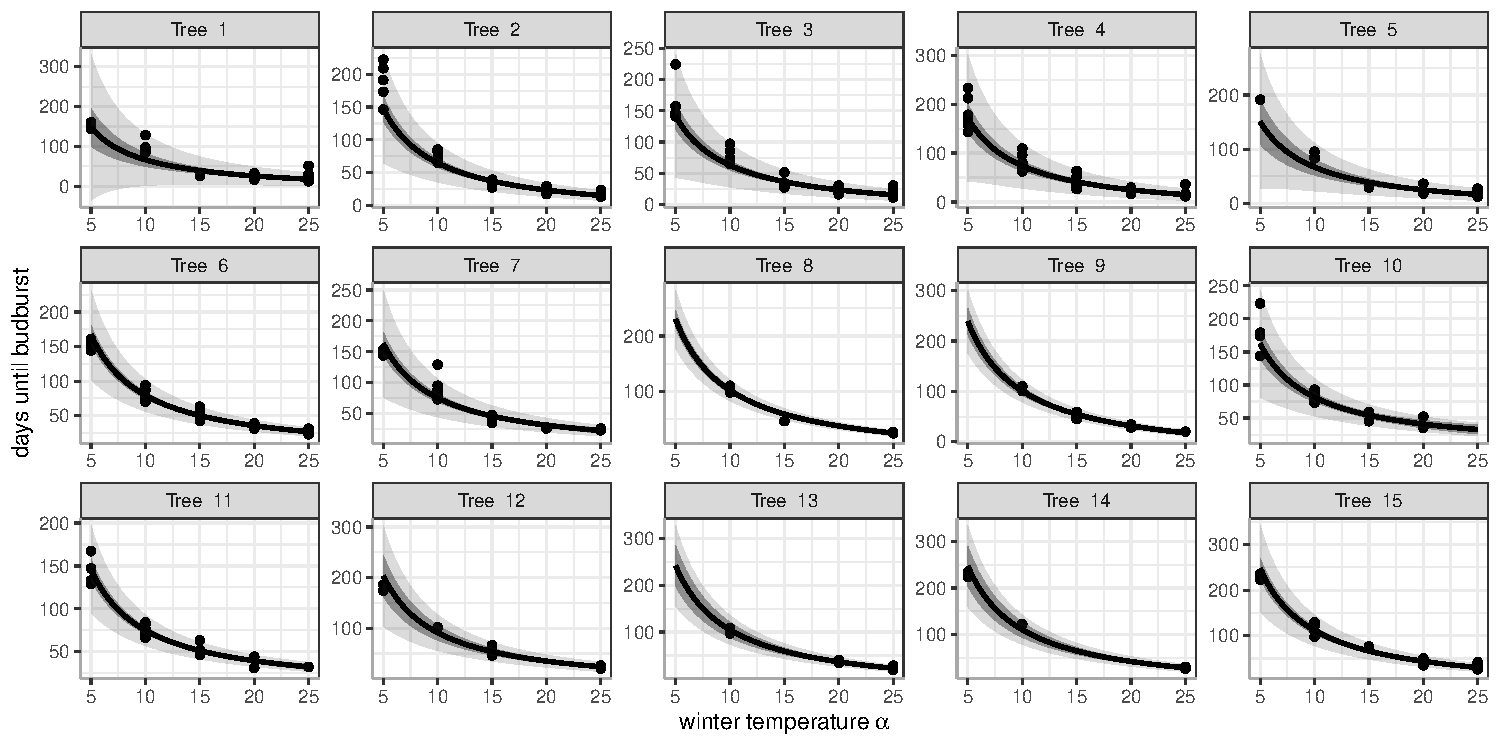
\includegraphics[width=1\linewidth]{figure-latex/experiment2} \caption{Mean time until budburst as a function of winter temperature ($\alpha$) in a controlled experiment conducted by Charrier et al. (2011) in which 385 buds were observed on stems sampled from 15 walnut trees (\textit{Juglans regia} and \textit{Juglans regia x nigra} hybrids), chilled at \(4^\circ\)C, and then warmed in different temperatures environments (x-axis) with the same photoperiod conditions across temperatures until budburst. For each tree (panel), we show the observed dates (points) and the fitted winter regime approximation of the thermal-sum model (the solid line denotes the mean, the inner grey region denotes the 95\% confidence interval of approximately two standard errors, and the outer grey region denotes the 95\% prediction interval of approximately two standard deviations). The figure highlights that the mean and variance are nonlinear functions of temperature even when biological factors such as chilling and photoperiod are held fixed. Both decrease with increasing temperatures as predicted by the thermal-sum model in the winter regime.} 
\label{fig:experiment}
\end{figure*}

% emwOct: If you want ONE more place to say 'plants and animals', you could do it below -- chuinearees is about process-based modeling for plants and animals
Our results show that the long-standing and widely-used thermal-sum model \citep{quetelet1849letters, chuinearees}\R{alreadycited2} explains observed shifts in the timing of biological events including declining sensitivity and synchrony. This finding has two important consequences. First, it challenges an extensive body of work that has attempted to revise the thermal-sum model by adding additional factors or mechanisms \citep{fu2015declining,kovaleskipreprint,piao2017,meng2020}.\R{morecites2} These factors can influence the timing of biological events, but our work suggests they do not themselves explain current trends in sensitivity and synchrony. Further, additional factors can produce inaccurate forecasts when modeled incorrectly.

To understand the role played by any additional factors, the basic relationship between event time and temperature must be modeled correctly. For example, the literature often assumes a linear relationship between temperature and event time with constant variance, which we have shown is inconsistent with the thermal-sum model. Our framework provides a simple and transparent way to encode the thermal-sum model, on top of which complexity may be added and better studied.

The second consequence is that the thermal-sum model predicts a `scattered spring' or general desynchronization of springtime events as their timing moves closer to the winter solstice. We find that the synchrony of lilac bloom dates, a common indicator of spring, will decline in much of the Southern United States by the year 2100 under a high-warming scenario (SSP5-8.5): For example, were lilac planted across the South in 2050, the average time between blooms would be less than two weeks in 76\% of locations. By 2100, however, the average time will be less than two weeks in only 18\% of locations (Figure \ref{fig:forecast_south}, note that the synchrony of species with lower threshold $(\tau)$ may decline sooner). In many locations, the average time will increase by several weeks.

Absent some compensating mechanism, the long-standing and widespread thermal-sum model predicts that the timing of biological events across ecosystems---from crops to forests and from plants to insects---will in many cases become more variable, with potential cascading consequences for industry and natural ecosystems.


\begin{figure*}
    \centering

    \begin{subfigure}[b]{0.9\textwidth}
        \centering
	   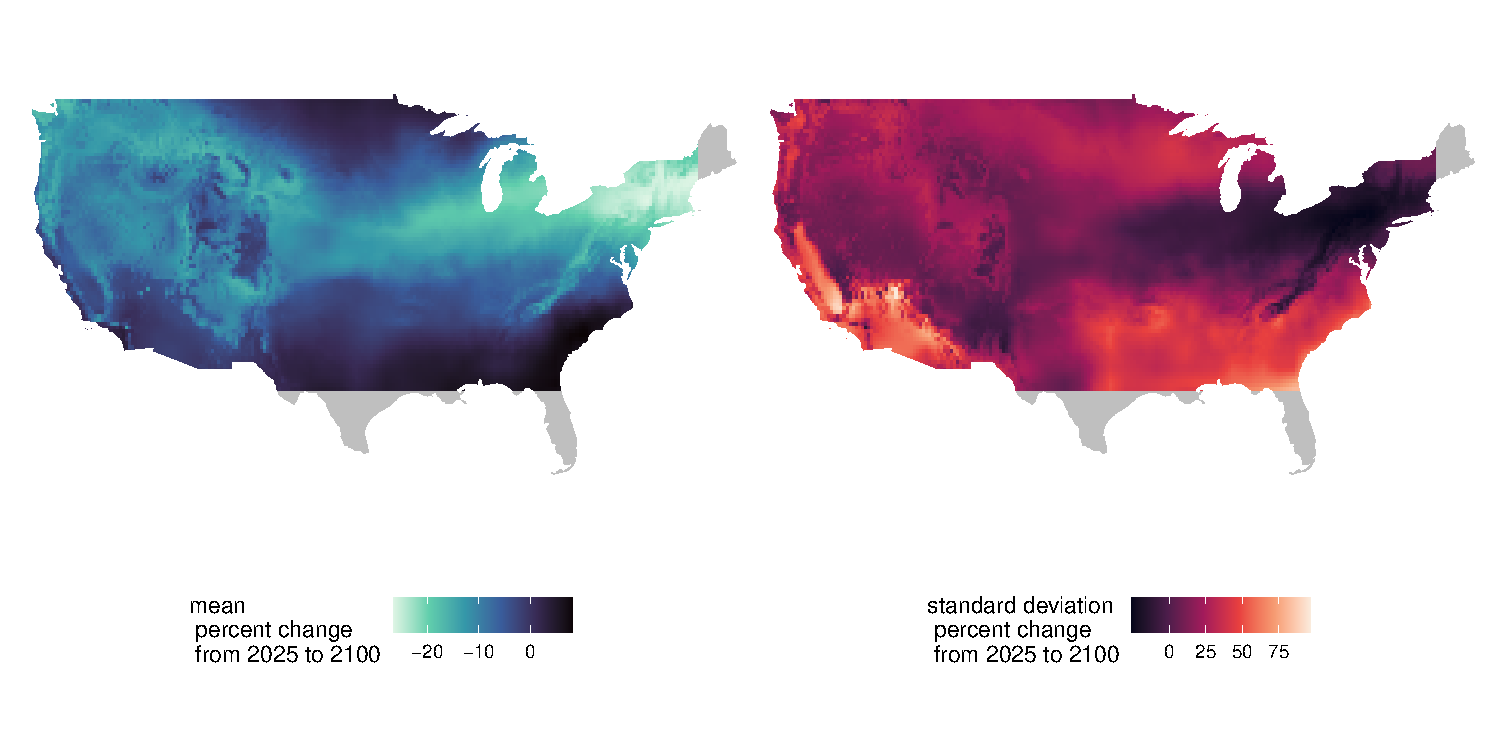
\includegraphics[width=1\linewidth]{figure-latex/forecast_pct_inc}
    \end{subfigure}

     \caption{Percent change in the mean (left) and standard deviation (right) of lilac bloom dates between the years 2025 and 2100 across the continental United States under temperatures projected in the NEX-GDDP-CMIP6  high-warming scenario SSP5-8.5 \citep{thrasher2022nasa}. Lighter areas indicate larger changes. The mean bloom date advances moderately, with the average bloom date occurring 20\% earlier in parts of the Northeast. In contrast, the standard deviation increases dramatically in some areas, with the average time between events increasing by 100\% in parts of the South, a phenomenon we refer to as a scattered spring.}
    \label{fig:forecast_south}
\end{figure*}

\newpage


% \noindent{The following Cell Press journals require most research articles to include their methods in a \textbf{METHODS} section, which should appear after the discussion: \textit{Cell Biomaterials}, \textit{Chem}, \textit{Chem Catalysis}, \textit{Cell Reports Physical Science}, \textit{Cell Reports Sustainability}, \textit{Device}, \textit{Joule}, \textit{Matter}, \textit{Newton}, \textit{One Earth}, and \textit{Patterns}. For all other Cell Press journals, please \textbf{delete} the contents of this page from the template and refer instead to \textbf{STAR Methods} on page 9.}

\section*{METHODS}

%%%  The methods (also/formerly called "experimental 
%%%  procedures") should appear 
%%%  immediately after the discussion. Subheadings 
%%%  may be customized. Please consult your handling 
%%%  editor if you have questions about what content 
%%%  should appear here. 


Our observational data analysis considers all sites in the historical lilac--honeysuckle phenology network \citep{rosemartin2015lilac} that recorded the phenophase full bloom and were within 10 miles of a Global Historical Climatology Network daily (GHCNd)  site with sufficiently complete temperature records. We limit our analysis to common lilac (\textit{Syringa vulgaris}), including all observations made from 1955 to 2025 as recorded by the USA National Phenology Network. The data were retrieved using the \texttt{R} package \texttt{rnpn}, resulting in \(10,613\) observations. 

For each observation, we estimate the winter temperature \((\alpha)\) using the average daily temperature between January and February, and we estimate spring warming \((\beta)\) using the slope of a linear regression model fit by regressing daily temperature on day index (i.e., $i=1$ for January 1, $i=2$ for January 2, etc.) over March and April (Figure S1, S2, and S3 in SI.3). Temperatures below \(0\) are set to \(0\), a common base temperature in growing degree day models. 

We then fit a two-parameter Gaussian location--scale model using the \texttt{gaulss} function from the \texttt{R} package \texttt{mgcv} in which we define 
\begin{align*}
 \mu(\alpha,\beta)&=\mathbb{E}[\nu(\tau) \mid \alpha,\beta] \\[1em]
 \sigma(\alpha,\beta)&=\mathrm{SD}(\nu(\tau) \mid \alpha,\beta).
 \end{align*} 
 Both \(\mu\) and \(\sigma\) are modeled with tensor-product splines with basis dimension k = 10 (Figure \ref{fig:lilac_te}). 
 
Finally, we calculate winter temperature $(\tilde \alpha)$ and spring warming $(\tilde \beta)$ for the years 2025, 2050, 2075, and 2100 using the NEX-GDDP-CMIP6 temperature projections for two scenarios: SSP2-4.5 and SSP5-8.5 \citep{thrasher2022nasa} (Figure S4 in SI.3). We also calculate the projected mean bloom date $ \mu(\tilde \alpha,\tilde \beta)$ and standard deviation $\sigma(\tilde \alpha, \tilde \beta)$ (Figure \ref{fig:forecast_south} and Figures S5 and S6 in SI.3).

\newpage

%%%  The following components should appear after the 
%%%  methods. 
%%%  For journals using STAR Methods, these components 
%%%  should appear immediately after the discussion 
%%%  (after any "limitations" or "conclusions" subsection 
%%%  within the discussion).

\section*{RESOURCE AVAILABILITY}

%%%  The resource availability section is required 
%%%  for all research articles. This component 
%%%  has 3 subsections: "lead contact," "materials 
%%%  availability," and "data and code availability." 
%%%  All 3 subsections must be included, even if no 
%%%  unique materials were generated in the study. 
%%%  Do not edit or change the names of the subheadings. 
%%%  No other subheadings or text are allowed in the 
%%%  resource availability section.

\subsection*{Lead contact}

%%%  Authors are required to designate a lead contact, 
%%%  who will be responsible for communication with 
%%%  the journal before and after publication and is 
%%%  the arbiter of disputes, including concerns 
%%%  related to reagents or resource sharing. Only 
%%%  one author can be named the lead contact, and 
%%%  only the lead contact’s information may be 
%%%  provided in this section.

Requests for further information and resources should be directed to and will be fulfilled by the lead contact, Jonathan Auerbach (jauerba@gmu.edu).

\subsection*{Materials availability}

%%%  This subsection must include a statement describing 
%%%  the availability of newly generated materials 
%%%  associated with the paper, including any conditions 
%%%  for access. If there are no newly generated materials 
%%%  associated with the paper, the statement should 
%%%  state this, e.g.: This study did not generate new 
%%%  materials.

This study did not generate new maerials.

\subsection*{Data and code availability}

%%%  All original research papers must include a 
%%%  comprehensive and accurate “data and code 
%%%  availability” statement within the “resource 
%%%  availability” component of the paper before it 
%%%  is accepted for publication. These statements 
%%%  are structured and consist of three bulleted 
%%%  components. Each component must be present.

\begin{itemize}
    \item  All data are documented in the author's GitHub repository, which is readily available upon request, and will be made publicly available via Zenodo, KNB or similar upon publication.
    \item  All code are documented in the author's GitHub repository, which is readily available upon request, and will be made publicly available via Zenodo, KNB or similar upon publication.
    \item Any additional information required to reanalyze the data reported in this paper is available from the lead contact upon request.    
\end{itemize}


\section*{ACKNOWLEDGMENTS}

%%%  Use this section to acknowledge contributions 
%%%  from non-authors and list funding sources, 
%%%  including grant numbers.

We thank G. Charrier for sharing data and V. Van der Meersch for helpful comments and suggestions.

\section*{AUTHOR CONTRIBUTIONS}

%%%  This component is required for most research papers. 
%%%  Mention each individual author with a statement 
%%%  outlining the contribution of each author to the work.

Conceptualization, writing, and editing, J.A., A.G. and E.M.W; methodology and investigation, J.A. and E.M.W.

\section*{DECLARATION OF INTERESTS}

%%%  This component is required for all articles, even 
%%%  if the authors have no competing interests; if 
%%%  this is the case, insert "The authors declare no 
%%%  competing interests." Please refer to the 
%%%  declaration of interests policy: 
%%%  https://www.cell.com/declaration-of-interests

The authors declare no competing interests.

%%% \section*{DECLARATION OF GENERATIVE AI AND AI-ASSISTED TECHNOLOGIES}

%%%  If generative AI and AI-assisted technologies 
%%%  were used in the writing process, this must 
%%%  be disclosed in the paper. This declaration 
%%%  does not apply to the use of basic tools for 
%%%  checking grammar, spelling, references, etc. 
%%%  If you have nothing to disclose, please do not 
%%%  include this component.

%%% During the preparation of this work, the author(s) used [NAME OF TOOL OR SERVICE] in order to [REASON]. After using this tool or service, the author(s) reviewed and edited the content as needed and take(s) full responsibility for the content of the publication.

\section*{SUPPLEMENTAL INFORMATION INDEX}

%%%  Supplemental information must be uploaded as 
%%%  separate files. In the main text, please list the 
%%%  files to be included in a brief index. For details, 
%%%  please review the supplemental information guidelines: 

%%%  Journals with a general "methods" section: 
%%%  http://www.cell.com/supplemental-information

%%%  Journals with STAR Methods: 
%%%  https://www.cell.com/STAR-supplemental-information

The Supplemental Information (SI) has the following sections

\begin{description}
  \item[SI.1] Stopped Random Walks in a Nutshell
  \item[SI.2] Sketch of Theoretical Results
  \item[SI.3] Tables S1-S3
  \item[SI.4] Figures S1-S6.
  \item[SI.5] Simulations with Figure S7 and Table S4
\end{description}

\newpage





\section*{MAIN FIGURE TITLES AND LEGENDS}

%%%  At final submission, figure files MUST be 
%%%  provided separately as high-resolution image 
%%%  files. All of the panels for a figure should 
%%%  be in the same file. Figures should have 
%%%  clear labels/file names (Figure 1, Figure 2, 
%%%  etc.). 

%%%  Figure titles and legends should be placed 
%%%  at the end of the main text. You do not 
%%%  need to place the figures, nor their titles 
%%%  and legends, within the main text. While 
%%%  typesetting your article, our team will 
%%%  place each figure in the best location 
%%%  based on the final layout and on your 
%%%  figure citations, e.g., (Figures 1A and 1B). 

%%%  Please review the figure guidelines before 
%%%  submitting your final materials: 
%%%  https://www.cell.com/figureguidelines.

\noindent 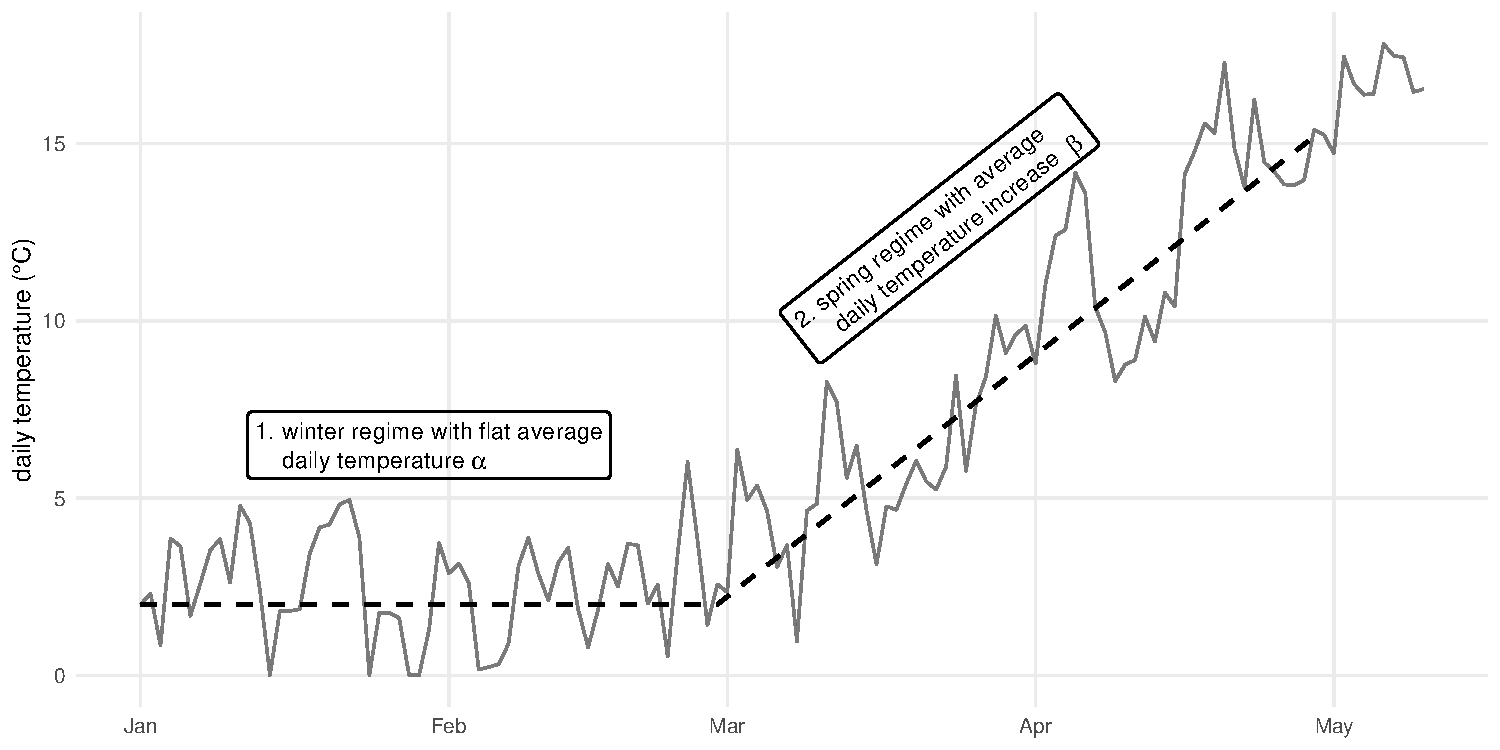
\includegraphics[width=0.9\textwidth]{figure-latex/two_regimes.pdf}

\subsection*{Figure 1. Temperature is flat near the winter solstice and increasing near the spring equinox.}

We model the daily temperature (solid line) as trend (dashed line) plus noise. The timing of springtime events in temperate climates depends on whether temperature is accumulated during one of two regimes, 1. the winter regime (relatively flat average daily temperature near the winter solstice, which we refer to as the `winter temperature' or $\alpha$), or 2. the spring regime (relatively linear average daily temperatures near the spring equinox, the slope of which we refer to as `spring warming' or $\beta$). We assume the effective temperature experienced by the bud is positive since biological limits prevent plants from accumulating very low forcing temperatures, taken here to be $0^{\circ}$C \citep{larcher1980} although this is easily adjusted.

\newpage 

\noindent \textbf{A} \vspace{-2em}  \newline 
\noindent 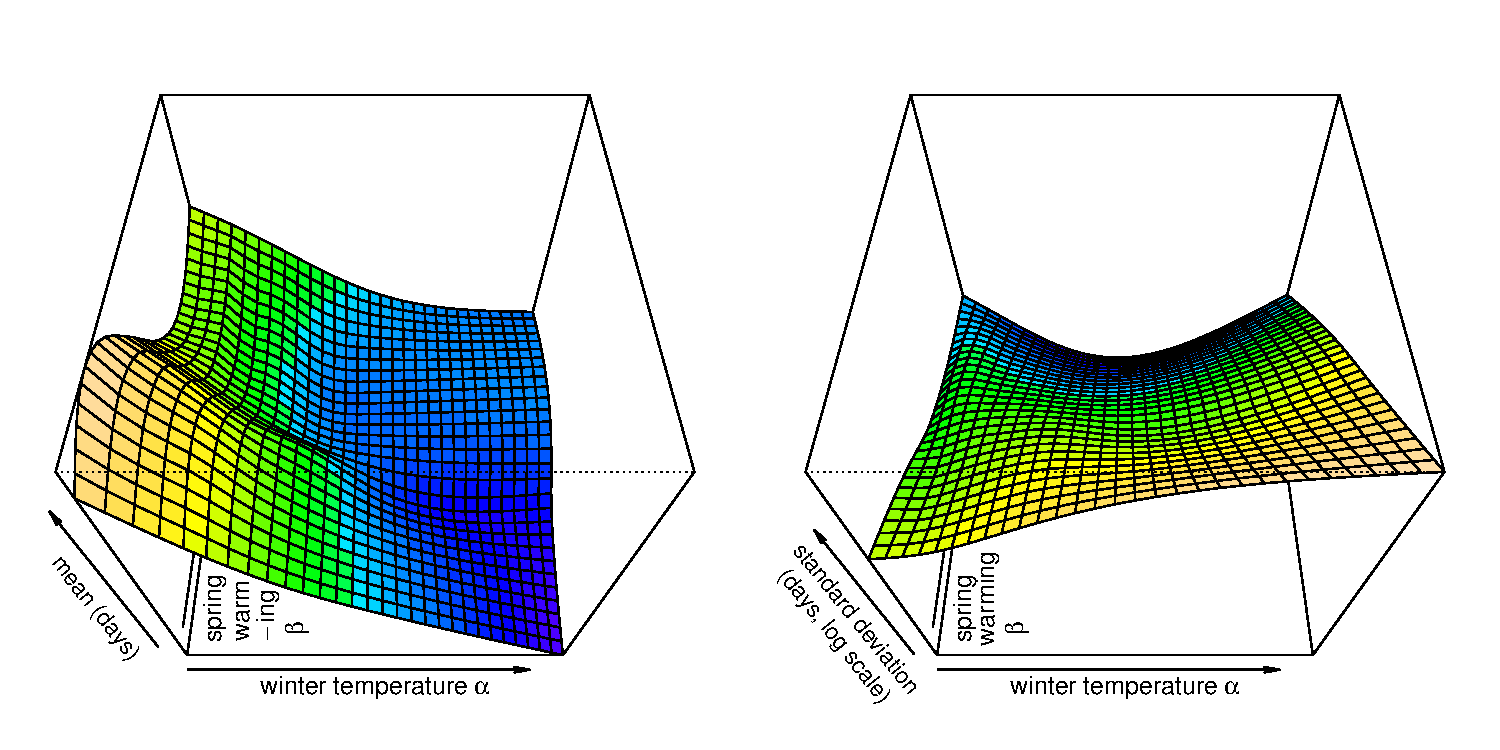
\includegraphics[width=1\linewidth]{figure-latex/lilac_te_mean-1}
\textbf{B}  \newline   \vspace{-2em} 
\noindent  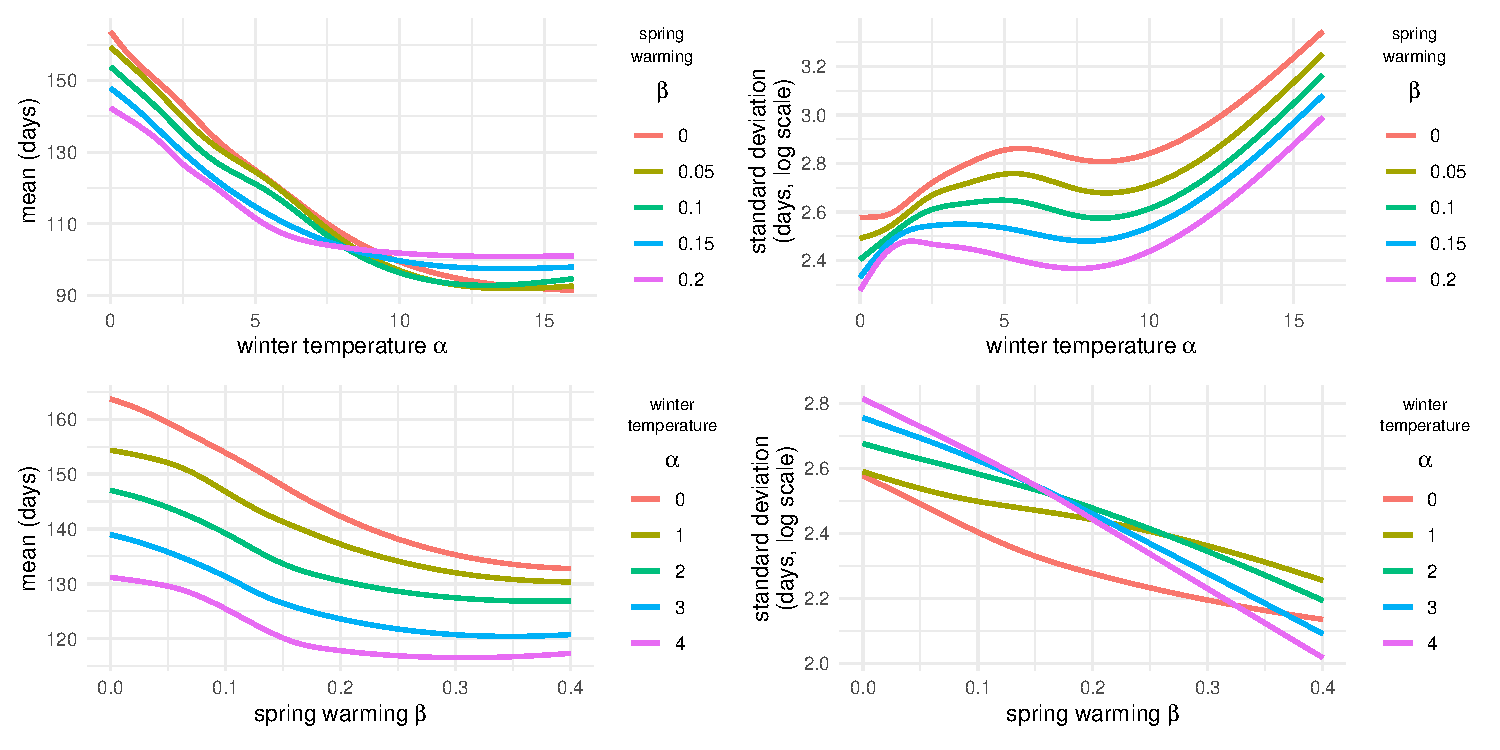
\includegraphics[width=1\textwidth, trim=0 0 .85in 0, clip]{figure-latex/lilac_te_mean-2_t}

\subsection*{Figure 2. Lilac bloom dates as modeled by a generalized additive model.}

Mean and log standard deviation of lilac bloom dates (n = 10,613 from Rosemartin et al. 2015, updated to 2025 using USA National Phenology Network records) by winter temperature $(\alpha)$ and spring warming $(\beta)$ as estimated by a generalized additive model. The estimated functions are shown using bivariate plots (\textbf{A}) and cross-section plots (\textbf{B}). The bivariate plots show the mean decreases as $\alpha$ and $\beta$ increase (left), while the standard deviation can increase or decrease depending on the relative values of $\alpha$ and $\beta$ (right). The cross-section plots show the mean decreases both as \(\alpha\) increases holding \(\beta\) constant (top left) and as \(\beta\) increases holding \(\alpha\) constant (bottom left), while the standard deviation increase when \(\alpha\) increases holding \(\beta\) constant (top right) and decreases when \(\beta\) increases holding \(\alpha\) constant (bottom right). Temperature is measured in $^\circ$C.

\newpage 

\noindent 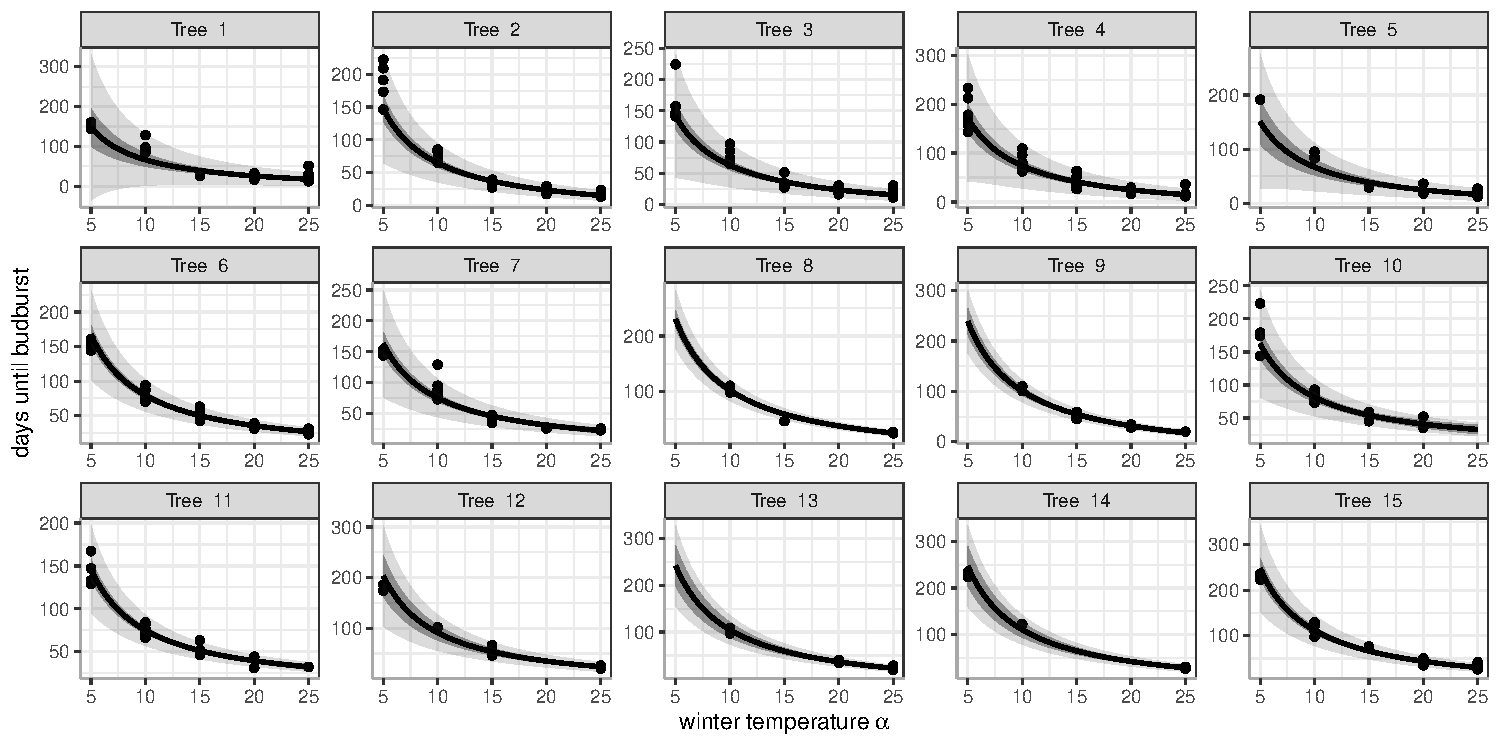
\includegraphics[width=1\linewidth]{figure-latex/experiment2} 

\subsection*{Figure 3. Walnut tree leafout dates from a controlled experiment.}

Mean time until budburst as a function of winter temperature ($\alpha$) in a controlled experiment conducted by Charrier et al. (2011) in which 385 buds were observed on stems sampled from 15 walnut trees (\textit{Juglans regia} and \textit{Juglans regia x nigra} hybrids), chilled at \(4^\circ\)C, and then warmed in different temperatures environments (x-axis) with the same photoperiod conditions across temperatures until budburst. For each tree (panel), we show the observed dates (points) and the fitted winter regime approximation of the thermal-sum model (the solid line denotes the mean, the inner grey region denotes the 95\% confidence interval of approximately two standard errors, and the outer grey region denotes the 95\% prediction interval of approximately two standard deviations). The figure highlights that the mean and variance are nonlinear functions of temperature even when biological factors such as chilling and photoperiod are held fixed. Both decrease with increasing temperatures as predicted by the thermal-sum model in the winter regime.


\newpage

\noindent  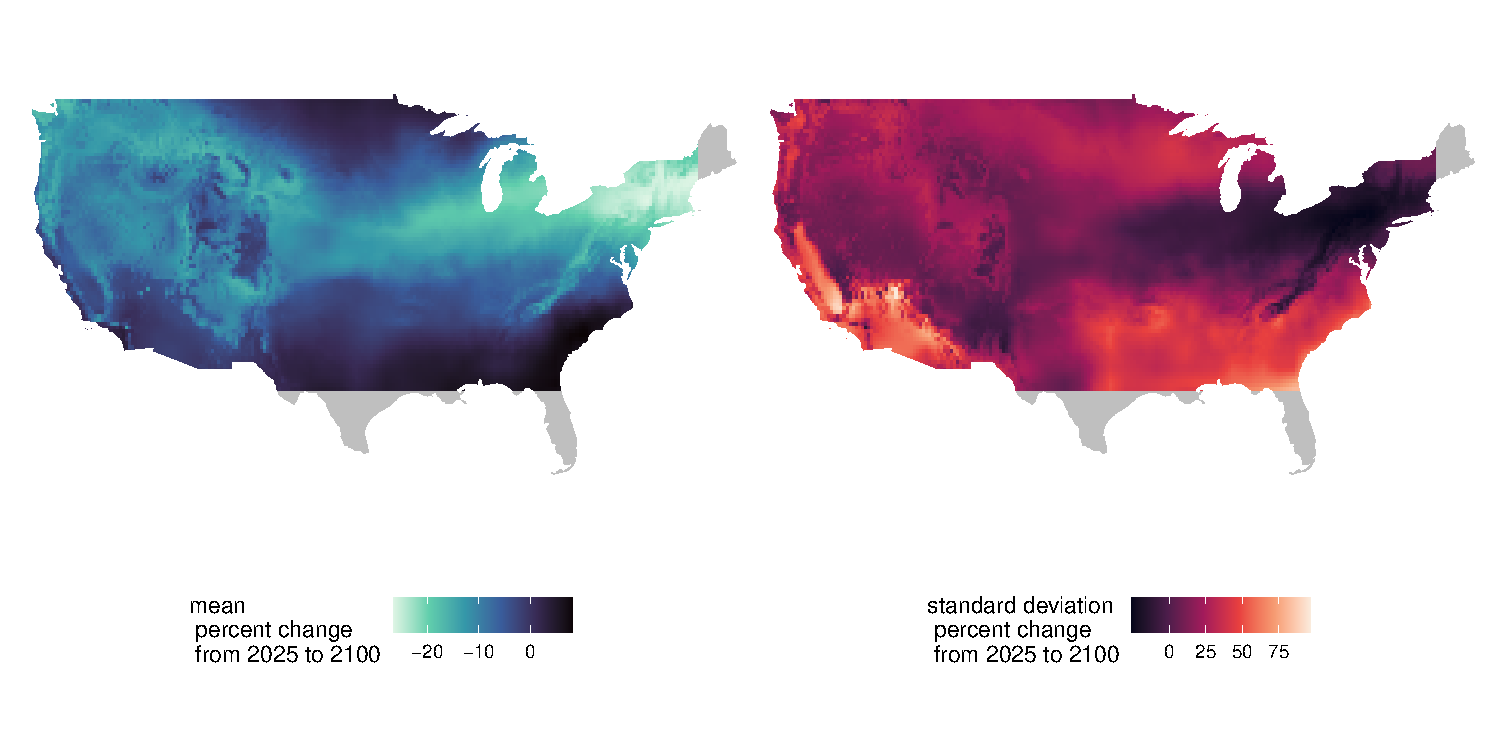
\includegraphics[width=1\linewidth]{figure-latex/forecast_pct_inc}

\subsection*{Figure 4. Projected mean and variance of lilac bloom dates under a high-warming scenario.}

Percent change in the mean (left) and standard deviation (right) of lilac bloom dates between the years 2025 and 2100 across the continental United States under temperatures projected in the NEX-GDDP-CMIP6  high-warming scenario SSP5-8.5 \citep{thrasher2022nasa}. Lighter areas indicate larger changes. The mean bloom date advances moderately, with the average bloom date occurring 20\% earlier in parts of the Northeast. In contrast, the standard deviation increases dramatically in some areas, with the average time between events increasing by 100\% in parts of the South, a phenomenon we refer to as a scattered spring.


\newpage

%%%  REFERENCES: As of 2023, all Cell Press journals 
%%%  use Numbered (AMA) style. We recommend placing 
%%%  your references in the included "references.bib" 
%%%  file.


\bibliography{auerbach_gelman_wolkovich}



\bigskip

%%%  In your References, please include only articles 
%%%  that are published (online publication and 
%%%  preprint servers are OK). Unpublished data, 
%%%  submitted and/or accepted manuscripts, abstracts, 
%%%  and personal communications should be cited within 
%%%  the text only ("unpublished data," "data not 
%%%  shown," "Alice Smith, personal communication") 
%%%  and not included in the references list. Personal 
%%%  communication should be documented by a letter 
%%%  of permission. Whenever possible, please make 
%%%  sure your .bib file has the complete author lists 
%%%  for each item (at minimum, the first 11 authors 
%%%  listed). 

\end{document}

\newpage

All Cell Press \textbf{life and medical science} journals, and the multidisciplinary journal \textbf{iScience}, use the \textbf{\href{https://www.cell.com/star-authors-guide}{STAR Methods}} format for reporting materials and methods. Other Cell Press journals use a non-structured \textbf{methods} format; for those journals, please \textbf{delete} the contents of this page from the template and refer instead to the \textbf{methods} template on page 3.

If you are publishing in a STAR Methods journal, please refer to the appropriate guide for authors:
\begin{itemize}
\item \textit{Cell} authors should download the guide for \textit{Cell} authors \href{https://www.cell.com/pb-assets/journals/research/cell/methods/Methods_Guide_Cell-1678470557763.pdf}{available here}
\item All other journal authors should use \href{https://www.cell.com/pb-assets/journals/research/cell/methods/Methods_Guide_general-1678470557763.pdf}{this version of the guide}
\end{itemize}


\section*{STAR METHODS}

%%%  The STAR Methods should appear in your main 
%%%  manuscript file after the figure legends, main 
%%%  table(s) and table legend(s).

\subsection*{Key resources table}

\textit{To create the KRT, please use the \href{https://star-methods.com}{KRT webform} or the \href{http://www.cell.com/pb-assets/journals/research/cell/methods/table-template1.docx}{Word template} and upload this file separately.}

\subsection*{Experimental model and study participant details}

%%%  Please list here under separate headings 
%%%  all the experimental models/study participants 
%%%  (animals, human participants, plants, microbe 
%%%  strains, cell lines, primary cell cultures) 
%%%  used in the study. For each model, provide 
%%%  information related to their species/strain, 
%%%  genotype, age/developmental stage, sex (and 
%%%  gender, ancestry, race, and ethnicity if 
%%%  reported for human studies), maintenance, 
%%%  and care, including institutional permission 
%%%  and oversight information for the studies 
%%%  the experimental animal/human participant 
%%%  study. The influence (or association) of sex, 
%%%  gender, or both on the results of the study 
%%%  must be reported. In cases where it cannot, 
%%%  authors should discuss this as a limitation 
%%%  to their research’s generalizability.

%%%  Please omit this component if your study does 
%%%  not use experimental models typical in the 
%%%  life sciences (e.g., if your study is 
%%%  computational or physical science research). 

\subsection*{Method details}

%%%  Please provide precise details of all the 
%%%  procedures in the paper (behavioral task, 
%%%  generation of reagents, biological assays, 
%%%  modeling, etc.) such that it is clear how, 
%%%  when, where, and why procedures were 
%%%  performed. We encourage authors to provide 
%%%  information related to the experimental 
%%%  design as suggested by NIH and ARRIVE 
%%%  guidelines (e.g., information about 
%%%  replicates, randomization, blinding, sample 
%%%  size estimation, and the criteria for 
%%%  inclusion and exclusion of any data or 
%%%  subjects).

\subsection*{Quantification and statistical analysis}

%%%  Please describe here all statistical analysis 
%%%  and software used. We ask authors to indicate 
%%%  in this component where all of the statistical 
%%%  details of experiments can be found (e.g., in 
%%%  the figure legends, figures, results, etc.), 
%%%  including the statistical tests used, exact 
%%%  value of n, what n represents (e.g., number 
%%%  of animals, number of cells, etc.), definition 
%%%  of center, and dispersion and precision 
%%%  measures (e.g., mean, median, SD, SEM, confidence 
%%%  intervals). Also, please summarize in this 
%%%  component how significance was defined, the 
%%%  statistical methods used to determine strategies 
%%%  for randomization and/or stratification, sample 
%%%  size estimation, and inclusion and exclusion 
%%%  of any data or subjects, as well as any methods 
%%%  used to determine whether the data met 
%%%  assumptions of the statistical approach.

\subsection*{Additional resources}

%%%  Please provide links to websites that provide 
%%%  further information relevant to the study 
%%%  (e.g., protocol download, troubleshooting 
%%%  forum, etc.). Clinical trial registry numbers 
%%%  and links should also be placed here. Please 
%%%  briefly describe the resource and its 
%%%  relevance for the paper. Please report this 
%%%  information as: “Description: URL.”

 Cell.com homepage: https://www.cell.com
 \newline Templates for Cell Press authors: https://www.cell.com/article-templates

%%%  ADDITIONAL MANUSCRIPT COMPONENTS:

%%%  Depending on the journal and the article 
%%%  type, you may be asked to upload the 
%%%  following as separate files: graphical 
%%%  abstract, highlights, eTOC blurb (In 
%%%  Brief), and/or other article components 
%%%  such as a "bigger picture" statement. 
%%%  These items are typically not required for 
%%%  initial submissions. Please refer to the 
%%%  journal's website, your acceptance 
%%%  letter, and/or the Final Files 
%%%  Requirements checklist to see if any of
%%%  these items are required (at any stage).
